%----------------------------------------------------------------------------------------
%	PACKAGES AND THEMES
%----------------------------------------------------------------------------------------
\documentclass[aspectratio=169,xcolor=dvipsnames, t]{beamer}
\usepackage{fontspec} % Allows using custom font. MUST be before loading the theme!
\usetheme{SimplePlusAIC}
\usepackage{ulem} 
\usepackage{hhline}
\usepackage{hyperref}
\usepackage{graphicx} % Allows including images
\usepackage{booktabs} % Allows the use of \toprule, \midrule and  \bottomrule in tables
\usepackage{svg} %allows using svg figures
\usepackage{tikz}
\usepackage{makecell}
\usepackage{amsmath} % For \textsubscript command
\usepackage[english]{babel}
\usepackage[backend=biber, style=apa]{biblatex}
\addbibresource{test.bib}
\usepackage{wrapfig}
% ADD YOUR PACKAGES BELOW
\usetikzlibrary{calc,patterns.meta}
\usepackage{totcount}
\regtotcounter{section}
\usepackage{forest}

\usepackage{colortbl}
\usepackage{color,soul}
\usepackage{xcolor}
\usepackage{nameref}
% Redefinition of the \section command so that each one is labeled \label{sec:n} where n is its index 
\let\oldsection\section
\renewcommand{\section}[2][\relax]{%
    \ifx#1\relax
      \oldsection{#2}%
    \else
      \oldsection[#1]{#2}%
    \fi%
    \label{sec:\thesection}%
}

% Definition of custom colors based on the initial figure of the bar by the OP
\definecolor{myblue}{HTML}{57AED1}
\definecolor{mygreen}{HTML}{8BC53F}
\definecolor{mygray}{HTML}{DDDDDD}
\definecolor{BlueIuss}{HTML}{033354}
\definecolor{LightBlueIuss}{HTML}{1b4a74}

% Definition of custom tikz styles in order to ease readability
\tikzset{
    % Bar style (Argument : color)
    sectionbar/.style={
        % Filling with one color as a preaction, in order to avoid reset by the pattern color
        preaction={fill=#1!70},
        % Application of the line pattern on to of the fill
        pattern={Lines[angle=45,distance={6pt},line width=3pt]},pattern color=#1
    },
    % Node style (Arguments : color, section number)
    sectionnode/.style 2 args={
        fill=#1,
        draw=white,
        thick,
        circle,
        text=white,
        radius=10pt,
        % Display of the section name below the cicle
        label={[text=#1, text width=2cm, align=center]below:\nameref{sec:#2}},
        }
}


% Actual definition of the colorbar based on Gonzalo Medina's initial proposal
\makeatletter
    \def\pbar@progressbar{} % the progress bar
    \newcount\pbar@tmpcnta% auxiliary counter
    \newcount\pbar@tmpcntb% auxiliary counter
    \newdimen\pbar@pbht %progressbar height
    \newdimen\pbar@pbwd %progressbar width
    \newdimen\pbar@tmpdim % auxiliary dimension
    \pbar@pbwd=\linewidth
    \pbar@pbht=4pt

% The progress bar
\def\pbar@progressbar{%
    \pbar@tmpcnta=\value{section} % tmpcnta stores the section number
    \pbar@tmpcntb=\totvalue{section} % tmbcountb sotres the total amount of sections
    \advance\pbar@tmpcntb by 1 % tmbcountb is advanced by 1 in order to have the last bar segment after the last node

    \begin{tikzpicture}[very thin]
        % Clipping scope to avoid tests for the bar dimensions
        \begin{scope}
        % Clipping path
        \path[rounded corners=2pt,clip] (0pt,{-\pbar@pbht/2}) rectangle (\pbar@pbwd,{\pbar@pbht/2});
        % Gray bar (from 0 to last section)
        \path[sectionbar=mygray] (0pt,{-\pbar@pbht/2}) rectangle (\linewidth,{\pbar@pbht/2});
        % Blue bar (from 0 to the current section)
        \path[sectionbar=BlueIuss] (0pt,{-\pbar@pbht/2}) rectangle ({(\pbar@tmpcnta-0.5)*\linewidth/\pbar@tmpcntb},{\pbar@pbht/2});
        % Green bar (from current to next section)
        \path[sectionbar=LightBlueIuss] ({(\pbar@tmpcnta-0.5)*\linewidth/\pbar@tmpcntb},{-\pbar@pbht/2}) rectangle ({(\pbar@tmpcnta+0.5)*\linewidth/\pbar@tmpcntb},{\pbar@pbht/2});
        \end{scope}
        % Drawing of the nodes on top of the bars, based on the number of the current section
        \foreach \secnumber in {1,...,\totvalue{section}}{
            % Number is lower, section is past, blue color
            \ifnum\secnumber<\pbar@tmpcnta
                \node[sectionnode={BlueIuss}{\secnumber}] at ({(\secnumber-0.5)*\linewidth/\pbar@tmpcntb},0) {\strut\secnumber};
            \fi
            % Number is equal, section is current, green color
            \ifnum\secnumber=\pbar@tmpcnta
                \node[sectionnode={LightBlueIuss}{\secnumber}] at ({(\secnumber-0.5)*\linewidth/\pbar@tmpcntb},0) {\strut\secnumber};
            \fi
            % Number is larger, to be done section, gray color
            \ifnum\secnumber>\pbar@tmpcnta
            \node[sectionnode={mygray}{\secnumber}] at ({(\secnumber-0.5)*\linewidth/\pbar@tmpcntb},0) {\strut\secnumber};
            \fi
        }
  \end{tikzpicture}%
}

\addtobeamertemplate{headline}{}
{%
  \begin{beamercolorbox}[wd=\paperwidth,ht=12.2ex,center,dp=1ex]{white}%
    \pbar@progressbar%
  \end{beamercolorbox}%
}
\makeatother

%----------------------------------------------------------------------------------------
%	TITLE PAGE CONFIGURATION
%----------------------------------------------------------------------------------------

\title[short title]{Bayesian Deep Learning} % The short title appears at the bottom of every slide, the full title is only on the title page
\subtitle{for Limited Data Prediction}


\author{SAHRAOUI TAREK ZIAD}
\institute[Short title]{\textbf{Supervisor:  Mrs.CHAOUCHE RAMDANE}
\newline
\newline

Computer Science Department
\newline
University of Abou Bekr Belkaid Tlemcen
}

% Your institution as it will appear on the bottom of every slide, maybe shorthand to save space

\date{\today} % Date, can be changed to a custom date

%----------------------------------------------------------------------------------------
%	PRESENTATION SLIDES
%----------------------------------------------------------------------------------------

\begin{document}
\maketitlepage
%\section{Overview}
\begin{frame}[t]{Overview}
    % Throughout your presentation, if you choose to use \section{} and \subsection{} commands, these will automatically be printed on this slide as an overview of your presentation
    \tableofcontents
\end{frame}

%-----------------------------------------------


% Section divider frame
\makesection{Inroduction to DL}

%------------------------------------------------
% Bullets

\begin{frame}{Bullet Points}
    \textbf{DL (Deep Learning)}
    \begin{itemize}
        \item Subset of machine learning that focuses on artificial neural networks with multiple layers.
        \item DL models can learn directly from raw data.
        \item DL models can be prone to overfitting.
        \item may require regularization techniques to generalize well.
        \item Popular DL frameworks include TensorFlow, PyTorch, and Keras.
    \end{itemize}
\end{frame}


\begin{frame}{}
    \begin{figure}
    \centering
    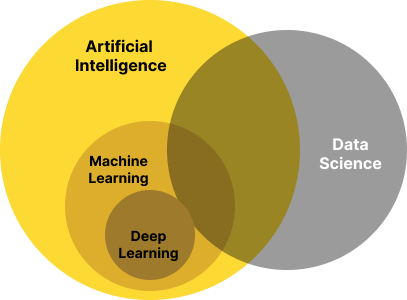
\includegraphics[width=0.6\textwidth]{Group 2.png}
    \caption{Venn diagram}
    \label{fig:example}
\end{figure}
\end{frame}

\begin{frame}{Bullet Points}
    \textbf{NN (Neural Networks)}
    \begin{itemize}
        \item Computational models inspired by the structure and function of biological NN.
    \end{itemize}
\end{frame}
\begin{frame}{}
    \begin{figure}
    \centering
    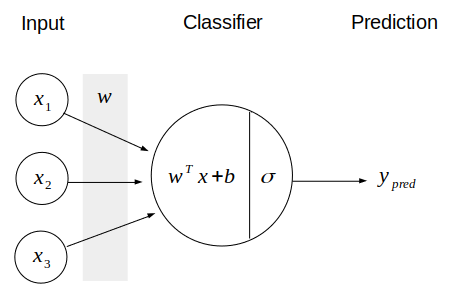
\includegraphics[width=0.6\textwidth]{images/ml-blog14-01.png}
    \caption{perceptron}
    \label{fig:example}
\end{figure}
\end{frame}


\begin{frame}{Bullet Points}
    \textbf{NN (Neural Networks)}
    \begin{itemize}
        \item Activation functions introduce non-linearities to the network.
        \item Neural networks encompass various types, such as (RNN) and (CNN).
    \end{itemize}
\end{frame}

\begin{frame}{}
    \begin{figure}
    \centering
    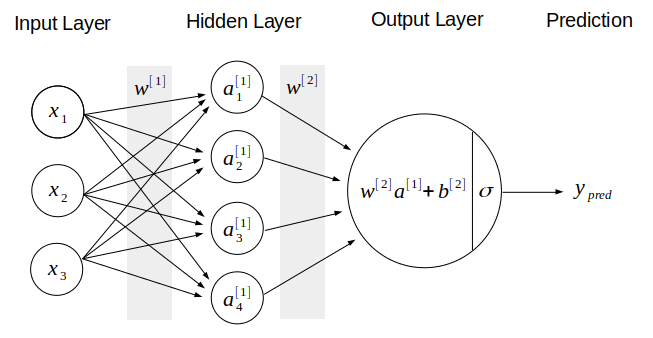
\includegraphics[width=0.8\textwidth]{images/ml-blog14-02.png}
    \caption{Neural network}
    \label{fig:example}
\end{figure}
\end{frame}





%------------------------------------------------
% Lists
\begin{frame}{Statistical Terms}
    \textbf{Bayes' Theorem}
    \begin{enumerate}
        \item Prior Distribution.
        \item Posterior Distribution.
        \item Likelihood.
    \end{enumerate}
    
    \textbf{Inference Techniques}
    \begin{enumerate}
        \item Variational Inference.
        \item Monte Carlo Dropout (MCD).
    \end{enumerate}
\end{frame}

\begin{frame}{Bayes' Theorem}
    \begin{figure}
        \centering
        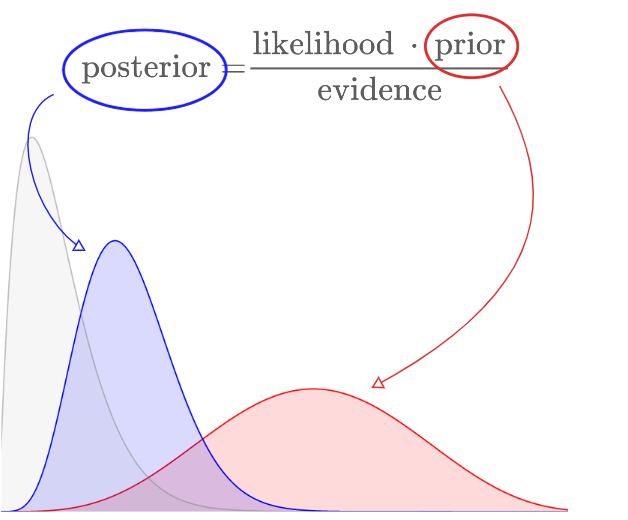
\includegraphics[width=0.8\textwidth,height=0.8\textheight,keepaspectratio]{Capture.PNG}
        \caption{Bayes' Theorem}
    \end{figure}
\end{frame}

\begin{frame}{Inference Techniques}
 \textbf{Variational Inference}
     \begin{enumerate}
        \item Approximate complex posterior distributions.
        \item Approximates the true posterior distribution.
        \item Trade-off between Accuracy and Efficiency.
        \item VI has applications in ML,NLP, CV, and computational biology.
    \end{enumerate}
\end{frame}

\begin{frame}{Inference Techniques}
\textbf{Monte Carlo Dropout}
     \begin{enumerate}
        \item MCD is based on the dropout regularization technique.
        \item Uncertainty Estimation.
        \item Provide more robust and calibrated predictions.
        \item MCD allows for the estimation of both (model uncertainty) and (data uncertainty).
    \end{enumerate}
\end{frame}
%------------------------------------------------


%------------------------------------------------
% Double columns
\begin{frame}{Monte Carlo Dropout}
    \begin{columns}
    \begin{column}{0.45\textwidth}
      \colheader{Dropout Regularization}
       
    \end{column}
    \begin{column}{0.45\textwidth}  %%<--- here
        \colheader{Explanation}
        technique where randomly selected neurons are ignored or "dropped out" during training.
    \end{column}
    \end{columns}
\end{frame}

\begin{frame}{Monte Carlo Dropout}
\begin{figure}
        \centering
        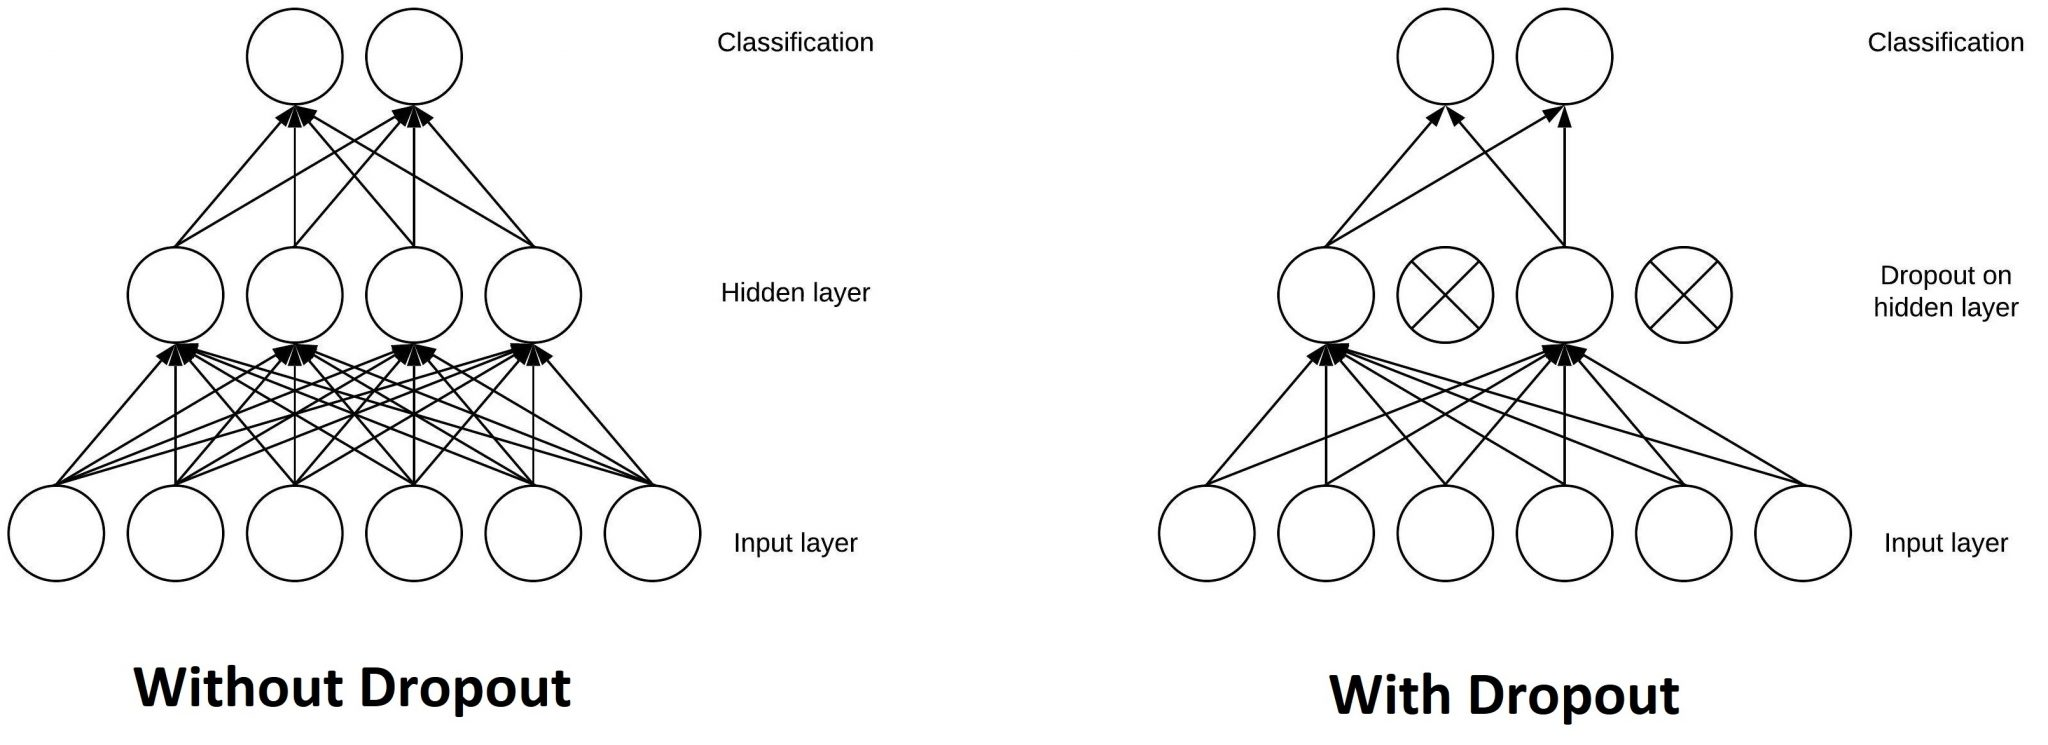
\includegraphics[width=0.8\textwidth,height=0.8\textheight,keepaspectratio]{images/dropout.jpg}
        \caption{DeepLearning  DropOut}
    \end{figure}
  
\end{frame}

%------------------------------------------------
% Table
\begin{frame}{Table}
    \begin{table}
        \begin{tabular}{l l l}
            \toprule
            \textbf{Treatments} & \textbf{Response 1} & \textbf{Response 2} \\
            \midrule
            Treatment 1         & 0.0003262           & 0.562               \\
            Treatment 2         & 0.0015681           & 0.910               \\
            Treatment 3         & 0.0009271           & 0.296               \\
            \bottomrule
        \end{tabular}
        \caption{Table caption}
    \end{table}
\end{frame}
%------------------------------------------------

% Section divider frame


\section{Motivation for BDL}

\begin{frame}{Bullet Points}
    \begin{itemize}
        \item Scarcity of Labeled Data.
    \end{itemize}
\end{frame}
\begin{frame}{Bullet Points}
    \begin{itemize}
        \item Scarcity of Labeled Data.
        \item Uncertainty Estimation.
    \end{itemize}
\end{frame}
\begin{frame}{Bullet Points}
  
\begin{figure}
        \centering
        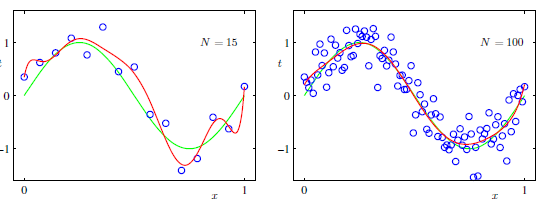
\includegraphics[width=0.8\textwidth,height=0.8\textheight,keepaspectratio]{images/regression.png}
        \caption{Uncertainty Estimation}
    \end{figure}
\end{frame}
\begin{frame}{Bullet Points}
    \begin{itemize}
     \item Scarcity of Labeled Data.
        \item Uncertainty Estimation.
        \item Robustness and Generalization.
    \end{itemize}
\end{frame}

\begin{frame}{Robustness and Generalization.}
    \begin{columns}
    \begin{column}{0.45\textwidth}
      \colheader{Robustness}
       
    \end{column}
    \begin{column}{0.45\textwidth}  %%<--- here
        \colheader{Explanation}
        refers to how well a model can maintain its performance under different conditions.
    \end{column}
    \end{columns}
\end{frame}
\begin{frame}{Robustness and Generalization.}
    \begin{columns}
    \begin{column}{0.45\textwidth}
      \colheader{Generalization}
       
    \end{column}
    \begin{column}{0.45\textwidth}  %%<--- here
        \colheader{Explanation}
        refers to how well a model can apply what it has learned from the training data to new, unseen data.
    \end{column}
    \end{columns}
\end{frame}



% Section divider frame
\makesection{Comparaison}

\begin{frame}{Used data}
    \begin{wrapfigure}{r}{0.4\textwidth}
    \centering
    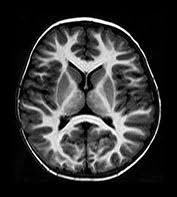
\includegraphics[width=0.4\textwidth]{images/14 no.jpg}
    \caption{Brain MRI Image}
\end{wrapfigure}
The dataset "Brain MRI Images for Brain Tumor Detection," uploaded by NAVONEEL CHAKRABARTY on Kaggle, comprises images of size 16MB, focusing on the concept of limited data with class labels "yes" and "no." 

\end{frame}


\begin{frame}{Used data}
    \begin{wrapfigure}{r}{0.4\textwidth}
    \centering
    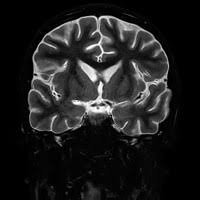
\includegraphics[width=0.4\textwidth]{images/19 no.jpg}
    \caption{Brain MRI Image}
\end{wrapfigure}
The training spanned 10 epochs and involved multiple models like VGG16, Simple CNN, Bayes by Backpropagation with L2 regularization and dropout (with changes to learning rate and regularization strength), traditional BNN and 2D CNN.

\end{frame}

\begin{frame}{Used data}
    \begin{wrapfigure}{r}{0.4\textwidth}
    \centering
    \includegraphics[width=0.4\textwidth]{images/3 no.jpg}
    \caption{Brain MRI Image}
\end{wrapfigure}
The dataset contained 178 images belonging to 2 classes and 75 images belonging to 2 classes. The study aimed to develop a brain tumor detection system utilizing these methods.

\end{frame}


\begin{frame}{Results}
   \begin{figure}[h]
    \centering
    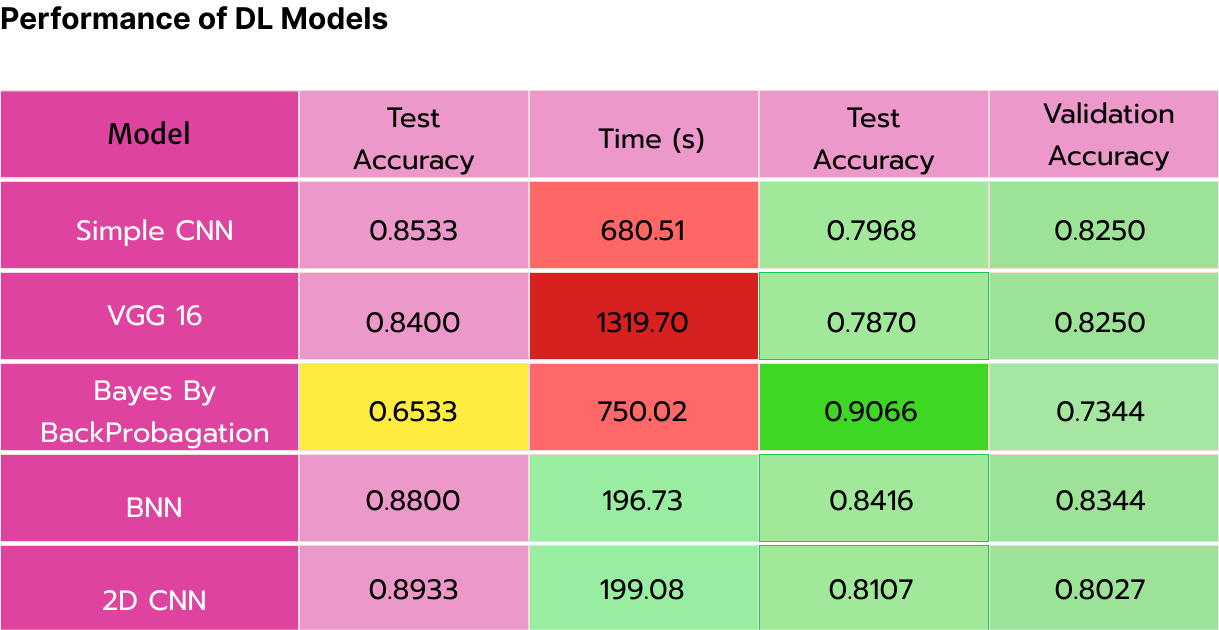
\includegraphics[width=0.8\textwidth]{images/table1.png}
    \caption{Example Image}
    \label{fig:example}
\end{figure}

\end{frame}


%------------------------------------------------
% Section divider frame
\makesection{Citations and References}

%------------------------------------------------
% Citations
\begin{frame}[fragile] % 
    \frametitle{Citation}
    An example of the \verb|\cite| command to cite within the presentation:\\~

    This statement requires citation \cite{rizzi_1976}.
\end{frame}

%------------------------------------------------
% Refenrenced
\begin{frame}[allowframebreaks]{References}
    % Beamer does not support BibTeX so references must be inserted manually as below
   %\printbibliography[heading=none]
\end{frame}

%----------------------------------------------------------------------------------------
% Final PAGE
% Set the text that is showed on the final slide
\finalpagetext{Thank you for your attention}
%----------------------------------------------------------------------------------------
\makefinalpage
%----------------------------------------------------------------------------------------
\end{document}